\documentclass[french,nochapter,11pt]{RapportProjet}
% Options chapter (1-) ou nochapter (2-)
%    1- la commande \chapter peut être utilisée dans le document (la classe report est chargée)
%    2- la commande \chapter NE peut PAS être utilisée dans le document (la classe article est chargée)
% Option nologo (à utiliser seulement si vous ne souhaitez pas afficher les logos sur la première page
%

\author{
    Corentin Banier \\
    Ibrahim El Umari \\
    Omar Jeridi \\
    Bilal Zaraket
}

\college{Polytech Nantes}
\course{Mini-Projet C++}
\academicyear{2022 - 2023}

\definecolor{mGreen}{rgb}{0,0.6,0}
\definecolor{mGray}{rgb}{0.5,0.5,0.5}
\definecolor{mPurple}{rgb}{0.58,0,0.82}
\definecolor{backgroundColour}{rgb}{0.95,0.95,0.92}
\lstdefinestyle{CPPStyle}{
    backgroundcolor=\color{backgroundColour},   
    commentstyle=\color{mGreen},
    keywordstyle=\color{magenta},
    numberstyle=\tiny\color{mGray},
    stringstyle=\color{mPurple},
    basicstyle=\footnotesize,
    breakatwhitespace=false,         
    breaklines=true,                 
    captionpos=b,                    
    keepspaces=true,                 
    numbers=left,                    
    numbersep=5pt,                  
    showspaces=false,                
    showstringspaces=false,
    showtabs=false,                  
    tabsize=2,
    language=C++
}

\linespread{1.2}

\begin{document}

\title{Rapport du projet}
\subject{\texttt{Dicewars}}
\maketitle

\section{Modèles d'objets}
\subsection{Générateur de carte}
La génération de la carte est inspirée du diagramme de Vorono\"i.\newline
\enquote{
    En mathématiques, un diagramme de Vorono\"i est un pavage (découpage) du plan en cellules (régions adjacentes) 
    à partir d'un ensemble discret de points appelés germes. 
    Chaque cellule renferme un seul germe, et forme l'ensemble des points du plan plus proches de ce germe que d'aucun autre. 
    La cellule représente en quelque sorte la zone d'influence du germe.
} (\url{https://fr.wikipedia.org/wiki/Diagramme_de_Vorono%C3%AF})

\begin{figure}[ht]
    \centering
    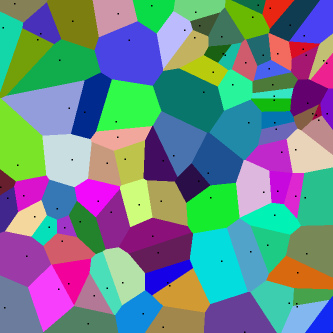
\includegraphics[width=10cm]{img/Coloured_Voronoi_2D.png}
    \caption{Diagramme de Vorono\"i}
    \label{fig:diagVoro}
\end{figure}

\subsection{Stratégie}
\label{sec:strat}
La stratégie que nous avons implémenté consiste à calculer la plus grande région du joueur, 
puis de lister toutes les cibles possibles. 
Nous faisons cela, car nous cherchons à maximiser le nombre de dés que l'on peut recevoir, 
et par conséquent, nous partons de notre plus grande région.
Nous trions cette liste à l'aide des facteurs suivants : 
\begin{enumerate}
    \item La différence de dés, nous favorisons les cibles faciles.
    \item Si la source d'attaque se situe dans la plus grande région alors on augmente la priorité.
\end{enumerate}

Pour résumer, la stratégie attaque les cibles les plus vulnérables et cherche à maximiser la plus grande région.\newline


\section{Spécificités dans l'implémentation}
\subsection{Générateur de cartes}
\subsubsection{Placement des germes}
\textit{Nous commençons par placer les germes \enquote{Seeds} dans la structure \texttt{Map} 
aléatoirement, en choisissant le nombre de \texttt{seeds} comme étant le \enquote{NbR}
puisque le nombre de germes représente aussi le nombre de régions obtenues à la fin.
}
\begin{lstlisting}[style=CPPStyle]
    // Choose a random set of seeds for the Voronoi diagram
    // by choosing always random seed we garuntee that its always a random map
    std::mt19937 rng;
    rng.seed(std::random_device()());
    std::uniform_int_distribution<std::mt19937::result_type> distX(0, mapWidth - 1);
    std::uniform_int_distribution<std::mt19937::result_type> distY(0, mapHeight - 1);
    const int numSeeds = c;  // number of seed also reflects number of regions
    std::vector<Territory> seeds;
    for (int i = 0; i < numSeeds; i++) {
      seeds.push_back(Territory(distX(rng), distY(rng), i));
    }
\end{lstlisting}
    
\subsubsection{Assignation des cellules aux régions}
\textit{Nous appliquons la simulation du diagramme de Vorono\"i afin d'assigner chaque cellule aux germes les plus proches.}
\begin{lstlisting}[style=CPPStyle]
    for (int x = 0; x < mapWidth; x++) {
        for (int y = 0; y < mapHeight; y++) {
            double minDistance = std::numeric_limits<double>::max();
            int closestSeed = -1;
            for (int i = 0; i < numSeeds; i++) {
                double d = distance(map[x][y], seeds[i]);
                if (d < minDistance) {
                    minDistance = d;
                    closestSeed = seeds[i].region;
                }
            }
            map[x][y].region = closestSeed;
        }
    }
\end{lstlisting}

\subsubsection{\enquote{Perçage} de la carte}
\textit{Les trois fonctions suivantes sont nécessaires afin d'ajouter du vide sur la carte : 
\texttt{removeRegion}, \texttt{findBorders} et \texttt{areNeighbors}}

\begin{lstlisting}[style=CPPStyle]
void removeRegion(std::vector<std::vector<Territory>>& map, int region);

std::vector<Territory> findBorders(const std::vector<std::vector<Territory>>& map);

bool areNeighbors(const std::pair<unsigned int, unsigned int>& t1, const std::pair<unsigned int, unsigned int>& t2);
\end{lstlisting}

\textit{Ces fonctions nous permettent de supprimer des régions tout en gardant la \texttt{Map} convexe.
Puis, nous supprimons au hasard des régions ( $\dfrac{nb\_regions}{5}$ ).
Nous vérifions qu'aucune région ne soit isolée.}

\subsubsection{Résultat}
\begin{figure}[ht]
    \centering
    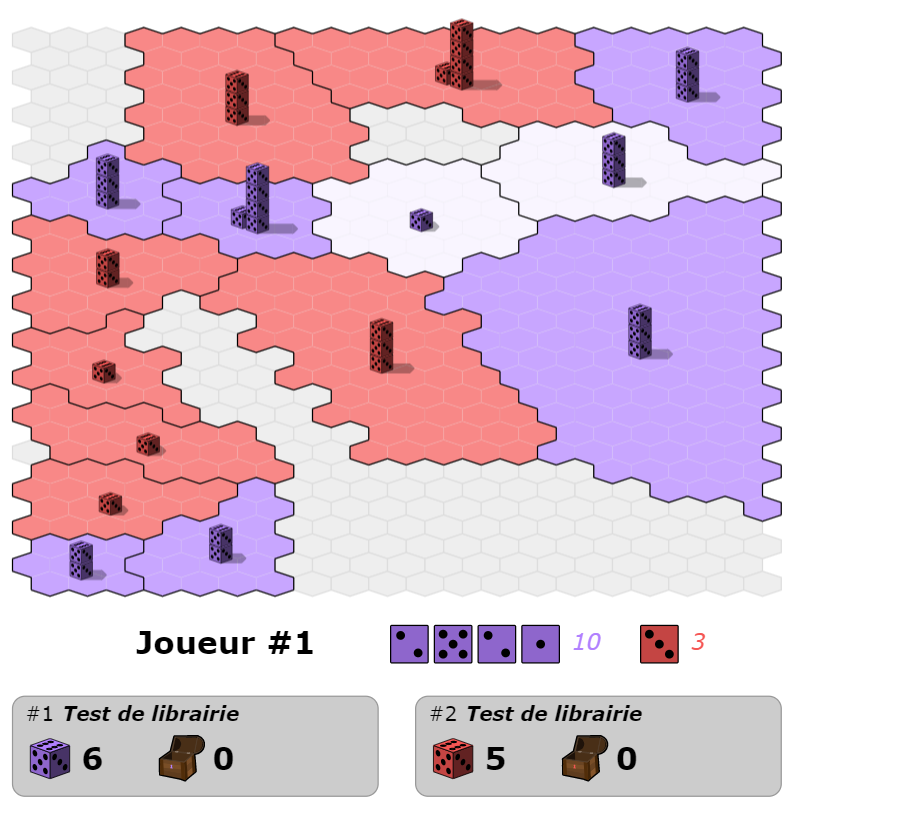
\includegraphics[width=10cm]{img/map.png}
    \caption{Exemple d'un carte}
    \label{fig:carte}
\end{figure}

\subsection{Stratégie}
\textit{Afin de regarder si un coup est autorisé, nous utilisons la fonction \texttt{isLegalMove}.
\begin{enumerate}
    \item La cellule de départ \texttt{from} doit avoir strictement plus de un dé.
    \item La cellule de départ \texttt{from} a au moins le même nombre de dés que dans la cellule attaquée \texttt{to}.
\end{enumerate}
}
\begin{lstlisting}[style=CPPStyle]
    bool isLegalMove(SMap& map,int Id,int from, int to);
\end{lstlisting}

\vspace{1.2em}

\textit{Structure contenant les cibles possibles, cette queue est triée par ordre de priorité, ainsi décrit dans la section \ref{sec:strat}.}
\begin{lstlisting}[style=CPPStyle]
    std::priority_queue<Attack,std::vector<Attack>,LessThanByDices> targets; 
\end{lstlisting}

\vspace{1.2em}

\textit{La fonction \texttt{getPossibleTargets} permet de remplir \texttt{priority\_queue} en prenant en compte la priorité.}
\begin{lstlisting}[style=CPPStyle]
    void getPossibleTargets(SMap& Map,int Id, std::set<int> biggestRegion, std::priority_queue<Attack, std::vector<Attack>, LessThanByDices>& targets);
\end{lstlisting}

\vspace{1.2em}

\textbf{Le tableau \texttt{regions} est très important dans les trois fonctions suivantes :}
\begin{enumerate}
    \item \textit{Divise les cellules appartenant au joueur d'une région (groupes de cellules connectées les unes aux autres et appartenant au même joueur)
    Pour éviter de tester une zone plusieurs fois, nous faisons appel à la fonction récursive \enquote{explore\_each\_region\_alone} pour atteindre toutes les cellules de chaque région.}
    \begin{lstlisting}[style=CPPStyle]
        void AggressiveAttackStrategy::Divide_into_regions();
    \end{lstlisting}

    \item \textit{La fonction récursive \texttt{explore\_each\_region\_alone} prend en paramètre un terrain, et l'ajoute dans la région \texttt{region\_number}.
    Puis, elle parcourt ses voisins afin de en trouver lesquels ont le même propriétaire et celles qui ne sont pas explorés.}
    \begin{lstlisting}[style=CPPStyle]
        void AggressiveAttackStrategy::explore_each_region_alone(int land, int *explored, int owner, int region_number);
    \end{lstlisting}

    \item \textit{La fonction \texttt{get\_largest\_region} boucle sur toutes les cellules dont nous sommes propriétaire 
    et détermine les autres régions qui ont le plus grand nombre de cellules connectées. La fonction retourne la plus grande région.}
    \begin{lstlisting}[style=CPPStyle]
        int AggressiveAttackStrategy::get_largest_region();
    \end{lstlisting}
\end{enumerate}

\clearpage

\section{Analyse}
\subsection{Analyse statique}
\begin{figure}[ht]
    \centering
    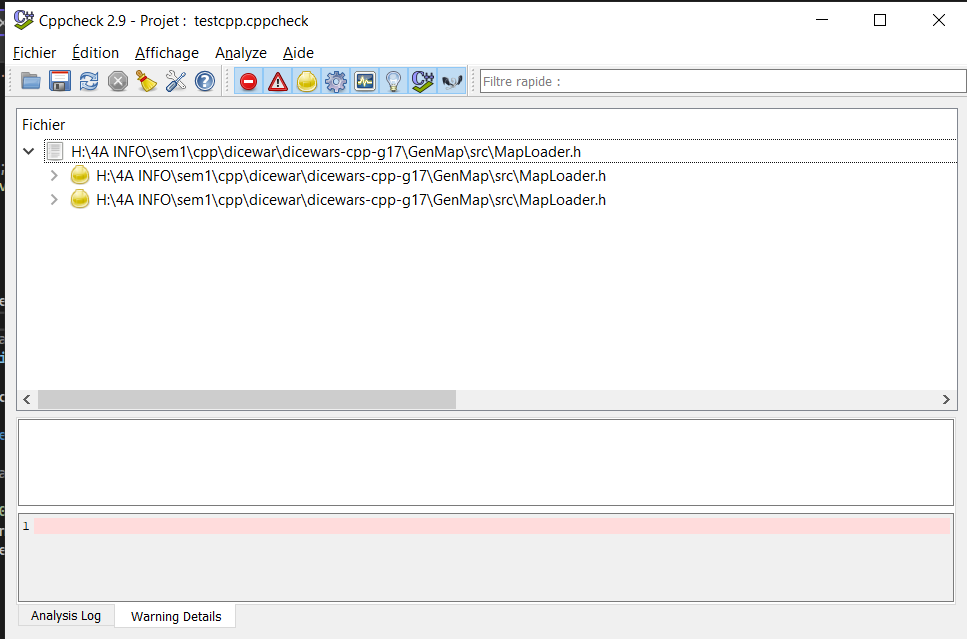
\includegraphics[width=14cm]{img/cppcheck.png}
    \caption{Résultat de \texttt{Cppcheck}}
    \label{fig:Cppcheck}
\end{figure}

\subsection{Analyse runtime}
Notre stratégie gagne toujours lorsqu'elle commence une partie.

\section{Remarques}
Nous avons également essayé de mettre en \oe uvre d'autres stratégies et d'ajouter d'autres fonctionnalités à notre stratégie, mais nous n'avons pas réussi à les implémenter.
Les voici : 
\begin{enumerate}
    \item Mise en place d'un algorithme pour connecter la région la plus grande à la région la plus proche de celle-ci afin d'augmenter la récompense en fin de tour 
    (déjà implémenté, mais pas placé sur la branche \texttt{master} à cause de bugs non résolus).
    
    Cette stratégie comporte deux approches :
    \begin{enumerate}
        \item La première approche est la plus rapide, où elle trouve juste le nombre minimum de terres nécessaires afin d'atteindre une autre région.
        \item La deuxième approche passe par la route ayant le nombre moyen minimum de dés.
    \end{enumerate}

    \item Un autre algorithme que nous avons implémenté, mais que nous avons ensuite supprimé, car il n'était pas assez efficace pour améliorer les performances de notre stratégie.
    Dans cette précédente stratégie, nous avions ajouté un facteur de faiblesse qui faisait que l'algorithme terminait son tour uniquement si le nombre de terrains ayant 
    un faible nombre de dés dépassait une certaine valeur seuil.
\end{enumerate}

\end{document}